\chapter{Technische Beschreibung}
In diesem Kapitel beschreibe ich die technische Umsetzung des Algorithmus, in ein konkretes C++ Programm.\\
Zunächst beginne ich mit einer allgemeinen Beschreibung der Implementation, gefolgt von einer Erklärung aller \textit{Objekte} und der Konzepte die diese umsetzen. Danach erfolgt eine genaue Beschreibung der Phasen und ihrer Teilschritte anhand von Pseudocode. Aus Gründen der Lesbarkeit und um unnötige Wiederholungen zu vermeiden, sind die Erläuterungen zum Umgang mit Kollisionen in den Hashmaps nicht in den Sektionen der Teilschritte, sondern in einem extra Abschnitt am Ende dieses Kapitels.\\
Die Begriffe \textit{\texttt{chain}}  und \textit{\texttt{group}} bezeichnen die in {\it Approximation LZ77 via Small-Space Multiple-Pattern Matching} beschriebenen theoretischen Konzepte.  \\
Dagegen beschreiben die Begriffe  Chain, Group und Factor  die C++ Objekte.

\section{Implementation}
Als Eingabe erhält die Implementation drei Werte:
\begin{itemize}
	\item einen zu komprimierenden Text \textit{T}
	\item eine zweier Potenz als maximale Größe der Faktoren $m$
	\item eine zweier Potenz  als minimal Größe der Faktoren $\theta$ kleiner gleich  $m$ 
\end{itemize} 
Der Algorithmus erstellt einen vollen Binärbaum über $T$, wobei jeder Knoten für einen Substring steht, den wir auf vorheriges Vorkommen untersuchen. Knoten mit vorherigen Substrings haben nie Kinder, während Knoten ohne vorherigen Substring immer zwei Kinder haben. Die Kinder eines Knoten symbolisieren das Prä- bzw. Suffix mit je halber Länge des Strings des Elternknotens. Aus diesen zwei Regeln ergibt sich die finale Struktur des Baumes.\\
%
%
In der Implementation beginnen wir damit, die Eingabe $T$ in die maximal größte gerade Anzahl an Teilstücke der Länge $m$ aufzuteilen. Zu jedem dieser Teilstücke erzeugen wir ein Chain Objekt. Diese repräsentieren die Knoten des Baumes auf der Ebene von der aus die weitere Bearbeitung erfolgt. Chains mit geradem Index sind immer linke Kinder und Chains mit ungeradem Index sind immer rechte Kinder. Die maximale Länge dieser Chains ist 32768, da sich dass Bereitstellen von mehr Speicher für größere Längen experimentell als nicht sinnvoll erwiesen hat.\\
%
%
Die Implementation untersucht alle Chains auf vorherige Substrings. Chains, die nicht gefunden wurden, ersetzen wir durch ihre zwei Kinder, die die Prä- bzw. Suffixe halber Länge darstellen. Ist eine Chain gefunden, löschen wir sie und speichern uns die gefundene Länge am verbleibenden Kind der Eltern Chain. Sollten beide Kinder gefunden worden sein, finden sie bei der weiteren Generierung des Baumes keine weitere Beachtung.
%
%
Das Programm bricht die Generierung des Baumes ab, sobald die Länge der Chains $\theta$ erreicht hat. In der Runde, in der wir Substrings der Länge $\theta$ untersuchen, generieren wir keine neuen Chains.\\
%PHASE 2
Der Algorithmus teilt nun alle Blätter des Baumes in  die sogenannten \textit{\texttt{chain}}  auf. Als Grenzen der \textit{\texttt{chain}}  dienen die cherrys, zwei Blätter mit gleichem Eltern Knoten. Eine aufsteigende \textit{\texttt{chain}}  besteht aus dem rechten Blatt der linken cherry und allen rechten Blättern des größtmöglichen Teilbaumes mit nur einer cherry. Eine absteigende \textit{\texttt{chain}}  besteht aus dem linken Blatt der rechten cherry und allen linken Blättern des größtmögliche Teilbaumes mit nur einer cherry.\\
\begin{figure}[h]
	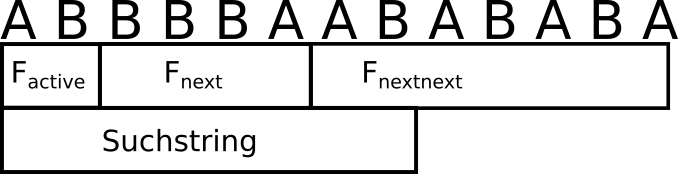
\includegraphics[width=0.8\textwidth]{Suchstring}
	\centering
		\caption{Entstehung des Suchstrings mit: |$F_{active}$|=2, |$F_{next}$|=4,|Suchstring|=8}
\end{figure}
\\
Die Implementation generiert aus jeder Chain, zu der mehr als ein gefundener Faktor assoziiert ist, ein Group Objekt.\\
Danach versucht der Algorithmus die Faktoren innerhalb der \textit{\texttt{chain}}  ausgehend von dem cherry Blatt zu mergen. Dazu markiert der Algorithmus in jeder \textit{\texttt{chain}}  das cherry Blatt als aktiv und testet ob es mit dem nächst größeren Faktor vereinigt wird. Das hängt davon ab ob ein vorheriger Substring für den Suchstring existiert. Der Suchstring besteht aus dem aktiven Faktor, dem nächsten Faktor und einem nicht leerem Prä- bzw. Suffix des übernächsten Faktors. Der Suchstring ist immer doppelt solang wie der nächste Faktor.\\ 
Sollte so ein vorheriger Substring existieren, mergen wir den aktiven und den nächsten Faktor, dieser neue Faktor ist nun aktiv. Existiert kein solcher Substring markieren wir den nächsten Faktor als aktiv.\\
Die Implementation folgt genau der zuvor beschriebenen Vorgehensweise. Wir markieren den kleinsten Faktor einer Group als aktiv und versuchen ihn mit dem nächsten Faktor zu mergen. Wir entscheiden dies genauso mit Hilfe eines Suchstrings der doppelt so lang ist wie der nächste Faktor.\\
Sowohl aus dem Algorithmus, als auch der Implementation erhalten wir so eine Menge an Faktoren, die eine 5-optimale LZ-Approximation darstellt.


\section{Objekte}
Im Folgenden beschreibe ich alle im Laufe der Bachelorarbeit entstandenen oder verwendeten Klassen.
C++ ist eine objektorientierte Programmiersprache, deren Vorzüge nur 
dann verständlich und nachvollziehbar erkennbar sind, wenn darin 
verwendete Objekt und Klassen  transparent dokumentiert werden. Die 
folgenden Beschreibungen beinhalten auch den in der Schreibweise 
ausgedrückten Bezug zur Implementation. Doppelbezeichnungen und 
Begriffe, die sowohl innerhalb der Implementation, wie auch im zu 
zugrundeliegenden Algorithmus verwendet werden, sind durch verschiedene 
Schreibweisen kenntlich gemacht.

\subsection{Chain}

\textit{Chain} Objekte stellen die im Algorithmus beschriebenen aktiven Knoten dar.
Jedes Chain Objekt enthält eine Position und eine Zahl die als Bitvektor interpretiert wird. Die Position der Chain gibt immer den Anfang des zu untersuchenden Substrings an. Der Bitvektor  gibt an welche gefundenen Längen mit der Chain assoziiert wurden. Zum Beispiel bedeutet ein gesetztes Bit an vierter Stelle, dass ein Faktor der Länge 16 gefunden wurde. \\
Eine Zahl mit einer Chain zu assoziieren oder eine Zahl zu einer Chain zu addieren, beschreibt das Setzten des entsprechenden Bits im Bitvektor. Dies wird durch einfache Veroderung ausgeführt.\\
Ein Chain Objekt ist damit 6 Byte groß.


\subsection{Group}

Ein \textit{Group} Objekt stellt die im Algorithmus beschriebenen \textit{\texttt{chain}} und einen aktiven Faktor dar.
Jedes Group Objekt enthält die Position, die Länge und die Quellposition des aktiven Faktors.
Außerdem besitzt eine Group eine Zahl die als Bitvektor interpretiert wird und  die die vor- bzw. zurückliegenden Faktoren darstellt. Dabei steht ein gesetztes Bit für einen Faktor der Länge wenn nur dieses Bit 1 wäre. Zusätzlich hat eine Group ein Flagbit, welches kennzeichnet ob es sich um eine aufsteigende oder absteigende \texttt{\textit{chain}} handelt.\\
Eine Group kann sich auf zwei Arten transformieren:
\begin{itemize}
	\item der nächste Faktor geht in die aktive Gruppe mit ein
	\item der aktive Faktor wird ausgegeben und der nächste Faktor wird aktiv
\end{itemize}
Ein Group Objekt ist 14 Byte groß.


\subsection{Factor}

Ein \textit{Factor} ist ein Triple aus drei Zahlen: der Position, der Länge und der Quellposition. 
Ein Faktor benötigt 12 Byte.

\subsection{Rollinghash}

Ein \textit{Rollinghash} Objekt besteht aus vier Werten: dem Hashwert, der Position, der Länge und dem Exponentenwert.
Der Hashwert enthält den Fingerprint des an Position beginnenden Substrings der gespeicherten Länge. \\
Ein Rollinghash dient dazu während der Suche über die Eingabe alle benötigten Werte zu verwalten.\\
Ein Rollinghash Objekt ist 24 Byte groß.


\section{Ablauf}

\subsection{Initialisation}

Die Initialisation beginnt damit die Fenstergröße anzupassen.
Sollte die maximale Faktorlänge, \textit{windowsize}, größer als der Text sein, so halbieren wir sie solange bis sie kleiner gleich  der Textlänge ist.
Ist die minimale Faktorlänge, \textit{threshold} $\theta$, größer als \textit{windowsize} $m$ brechen wir das ganze Programm ab.
Man könnte zwar einfach die Eingabe $T$ unkomprimiert ausgeben, aber da die Eingabewerte offensichtlich unlogisch sind, ist es sinnvoll hier das Programm mit einem Errorcode zu beenden.\\
Als nächstes erstellen wir die benötigten Container: einen Vektor für die zu bearbeitenden Chains $chainVec$, einen Vektor für die abgeschlossenen Chains  $p2\_buffer$, eine Hashmap für die Suche $hmap$, eine Hashmap für das Speichern der Quellpositionen $temp\_hmap\_store$ und einen Vektor, der diese zweiten Hashmaps speichert $hmap\_storage$.\\
Danach teilen wir die Eingabe \textit{T} in Teilstücke der Größe \textit{windowsize} auf.
Für jedes dieser Teilstücke, ausgenommen die letzten beiden, erzeugen wir ein Objekt vom Typ Chain und fügen es zu \textit{chainVec} hinzu.\\

\subsection{Phase 1}
Die erste Phase der Implementation erhält einen Vektor von Chains, die maximale Länge der Faktoren und die minimale Länge der Faktoren.\\
Als Ausgabe aus der ersten Phase erhalten wir zwei Vektoren aus Chains und einen Vektor von Hashmaps,  die mit allen gefundenen Quellpositionen gefüllt sind.\\

\noindent
In  Phase 1 simulieren wir das Erstellen des Baumes und der Bitvektoren in einer Schleife. Diese Schleife führen wir $\log_2{windowsize}-\log_2{threshold}$ mal aus. Zwei aufeinander folgende Chains im curr\_Chains stellen einen Knoten auf der momentanen Ebene des Baumes dar.
Wir füllen eine Hashmap $hmap$ mit key-value-pairs aus den Fingerprints und Indizes der Chains \autoref{Phase 1:2}.
Danach suchen wir mit einem Rollinghash Objekt über den Eingabetext $T$ und markieren gefundene Substrings \ref{Phase 1:3} \autoref{Phase 1:3}.
Als letzten Schritt in der Schleife entfernen wir Chains die \textit{cherrys} bilden und passen die noch zu bearbeitenden Chains an \autopageref{Phase 1:7}.
In der letzten Ausführung der Schleife überspringen wir diesen Schritt, da wir die Chains nicht für einen nächsten Durchlauf anpassen müssen \autopageref{Phase 1:6}. 
\begin{algorithm}[h!]
	\caption{Phase 1}
	\label{Phase 1}
	 \KwData{vector$<$Chain$>$ curr$\_$Chains, vector$<$Chain$> $phase2$\_$buffer, len$\_$t size, len$\_$t threshold, unordered$\_$map$<$uint64$\_$t, len$\_$t$>$ hmap,  unordered$\_$map$<$uint64$\_$t, len$\_$t$>$ temp\_hmap\_store, 
	 vector$<$unordered$\_$map$<$uint64$\_$t, len$\_$t$>>$ hmap\_store}
	\While{size>=threshold}
	{
		make$\_$hash$\_$map(hmap, temp\_hmap\_storage, curr$\_$Chains, size)\;\label{Phase 1:2}
		phase1$\_$search(hmap, curr\_Chains, size,
		temp\_hmap\_storage)\;\label{Phase 1:3}
		move temp\_hmap\_storage into hmap\_storage\;
		clear temp\_hmap\_storage and hmap\;
		\If{size>threshold\;\label{Phase 1:6}}{
			new$\_$and$\_$old$\_$chains(curr$\_$Chains, size, phase2$\_$buffer)\;\label{Phase 1:7}}
		
		size=size/2\;
	}
\end{algorithm}

\subsection{make$\_$hash$\_$map}
Die Funktion make$\_$hash$\_$map erhält eine Länge size, einen Vector mit Chains, einen Buffer für die zweite Phase, eine Hashmap die später zum Suchen benötigt wird und eine Hashmap, die die Quellpositionen abspeichert.\\
Die Funktion füllt die Hashmap mit den Fingerprints aller noch zu untersuchenden Chains und speichert alle bereits gefundenen Quellpositionen in einer zweiten Hashmap ab. Des Weiteren werden alle bereits gefundenen Chains mit der size assoziiert.\\

\noindent
Für jede Chain versuchen wir einen Eintrag in der Hashmap mit dem Fingerprint als Schlüssel und als Wert dessen Index im Vektor zu erstellen. Sollte aber schon ein Eintrag mit gleichem \textit{key} vorhanden sein, vergleichen wir zunächst unsere aktuelle $\text{Chain}_i$ mit der in der Hashmap vorhandenen \autopageref{makehash:2}. 
Wir addieren \textit{size} auf die Chain mit höherer Position und ändern den Hashmapeintrag auf den Index der Chain mit niedriger Position (Algo.2 L:6,8,9). Dies geschieht, weil ein vorher liegender Substring  eine Quellposition des späteren Faktors ist. Daher müssen wir nur noch nach dem vorherigen Substring suchen, da wir den anderen bereits gefunden haben.
Die gefundene Quellposition tragen wir in temp\_hmap\_storage unter dem entsprechenden Fingerprint ein (Algo.2 L:6,10), damit später nach der Quellposition nicht noch einmal gesucht werden muss.
\begin{algorithm}[ht!]
	\caption{make$\_$hash$\_$map}
	\label{makehash}
	\KwIn{vector$<$Chain$>$ chainVec, unordered$\_$map$<$uint64$\_$t, len$\_$t$>$ hashmap, unordered$\_$map$<$uint64$\_$t, len$\_$t$>$ temp\_hmap\_storage, len$\_$t size}
		\ForEach{$Chain_i$:chainVec}{
			\If{hashmap contains entry for fingerprint($Chain_i$)\;\label{makehash:2} }
			{
				hmap$\_$chain = chainVec[hashmap[fingerprint($Chain_i$)]]\;
				\If{hmap$\_$chain.position $<$ $Chain_i$.position}
				{$Chain_i$.add(size)\;
				temp\_hmap\_storage[fingerprint(hmap\_chain)]=hmap$\_$chain.position}	
				\Else
				{
					hmap$\_$chain.add(size)\;
					hashmap[fingerprint($Chain_i$)]=i\;
					temp\_hmap\_storage[fingerprint($Chain_i$)]=$Chain_i$.position\;
				}
			}
			\Else{add \{fingerprint($Chain_i$), i\} to hashmap\; }
		}
\end{algorithm}


\subsection{phase1$\_$search}
Die Funktion phase1$\_$search erhält die Liste aller Chains und eine Hashmap gefüllt mit den Fingerprints und  Indizes der zu überprüfenden Chains. Außerdem erhält die Funktion die Länge der Chains und eine leere Hashmap zum Speichern der Quellpositionen.\\
Am Ende der Funktion ist die zweite Hashmap mit allen gefundenen Quellpositionen gefüllt und alle Cherrys mit gefundener Quellposition wurden mit der size assoziiert.\\

\noindent
In phase1$\_$search suchen wir mit einem Rollinghash Objekt über den Text $T$.
Sollte die Hashmap einen Eintrag enthalten der dem Hashwert des Rollinghashes entspricht (Algo.3 L:3), so überprüfen wir ob der Rollinghash noch vor dem Substring liegt (Algo.3 L:5). Wenn dem so ist können wir \textit{size} auf die entsprechende Chain addieren.\\
Da wir als erstes das linkeste Vorkommen finden, liegt dies entweder vor dem Substring oder es ist der Substring selber. Daher müssen wir spätere Vorkommen nicht mehr betrachten und können deshalb den Eintrag aus der Hashmap entfernen(Algo.3 L:8).\\
Aus dem selben Grund fügen wir die Quellposition nur zu temp\_hmap\_store hinzu, wenn wir vor dem Faktor liegen, da wir sonst keine Quellposition gefunden haben (Algo.3 L:7).\\
Damit haben wir jede Chain deren aktueller Substring einen vorherigen Substring besitzt mit der aktuellen size markiert.
\begin{algorithm}[hbt!]
	\caption{phase1$\_$search}
	\KwIn{vector$<$Chain$>$ chainVec, unordered$\_$map$<$uint64$\_$t, len$\_$t$>$ hashmap, len$\_$t size}
	create Rollinghash Object of length size over the text $T$\;
	\While{rollinghash does not reach beyond $T$}
	{
		\If{hashmap contains entry for rollinghash.hashvalue}
		{
			chain = hashmap[rollinghash.hashvalue]\;
			\If{rollinghash.position<chain.position}
			{chain.add(size)\;
			temp\_hmap\_store[rollinghash.hashvalue]=rollinghash.position\;}
			
				
			hashmap.erase(rollinghash.hashvalue)\;
		}
			advance rollinghash\;
	
	}
\end{algorithm}

\subsection{new$\_$chains}
Die Funktion new$\_$chains erhält die Liste aller Chains und die Länge der untersuchten Substrings.\\
Am Ende der Funktion sind alle Chains die eine cherry bilden aus der Liste entfernt, für nicht gefundene Chains sind neue Chains eingefügt und gefundene Chains wurden entfernt. Alle Chains repräsentieren nun Substrings die halb so lang sind wie zuvor  \autoref{new chain}.\\

\noindent
Nachdem die Suche abgeschlossen ist müssen wir alle Chains untersuchen und feststellen, wie sie zu transformieren sind. Dies erfolgt immer in Zweierschritten, um die zusammengehörigen ab- und aufsteigenden Chains (dec, inc) gleichzeitig zu betrachten. Das heißt, wir betrachten immer eine Chain mit geradem Index und eine Chain mit ungeradem Index (0:1,2:3,4:5...). \\
Wir verunden bitweise die Bitvektoren von inc und dec mit der übergebenen Länge  und betrachten die Ergebnisse als \textit{Bool}werte.\\
\newpage
Für die Werte dec$\_$found und inc$\_$found gibt es damit vier mögliche Kombinationen:
\begin{outline}
	\1[]\texttt{dec$\_$found $\land$ inc$\_$found}:\\
		 Dieses Ergebnis bezeichnen wir als \textit{cherry}.\\
		 Beide Textstellen besitzen vorherige Substrings und beide Chains müssen in Phase 1 nicht weiter betrachtet werden. Wir verschieben inc und dec an das Ende von phase2$\_$buffer und ersetzen ihre Positionen durch die beiden letzten Chains im Vektor. Dies erspart uns, gegenüber dem Löschen, dass alle Chains im Vektor hinter inc und dec auch noch verschoben werden müssen.
		 Stammen diese beiden Chains bereits aus der vorherigen Runde (oder der Initialisation) so betrachten wir diese beiden als nächstes.
	\1[]\texttt{!dec$\_$found $\land$ !inc$\_$found}:\\
		In diesem Fall wurde kein Textstück gefunden das heißt, dass wir vier Kinder Chains haben müssen. Da wir bereits zwei Chains zur Verfügung haben (inc, dec)  passen wir diese einfach an und erstellen nur zwei passende neue Chains.
		Wir verschieben inc an das Ende des Vektors und fügen eine Kopie von inc am Ende des Vektors ein.
		Die Position dieser Kopie erhöhen wir um \textit{size}/2.
		Die alte Position von inc füllen wir durch eine Kopie von dec.
		Die Position dieser Kopie erhöhen wir um \textit{size}/2.\\
		Damit stehen die beiden Kinder von inc am Ende des Vektors und die beiden Kinder von dec an den ursprünglichen Positionen von dec und inc.
			
	\1[]\texttt{dec$\_$found $\land$ !inc$\_$found}:\\
		Wurde nur das linke Textstück gefunden, so ändern wir lediglich die Positionen von inc und dec.
		Inc nimmt die Position von dec an und wir erhöhen die Position von dec um \textit{size}/2.\\
		Damit stehen die beiden Kinder von inc an den ursprünglichen Positionen von dec und inc. 
	
	
	\1[]\texttt{!dec$\_$found $\land$ inc$\_$found}:\\
	Wurde nur das rechte Textstück gefunden, so ändern wir lediglich die Positionen von dec.
	Dec nimmt die Position von inc an und wir erhöhen die Position von dec um \textit{size}/2.\\
	Damit stehen die beiden Kinder von dec an den alten Positionen von dec und inc.
		
\end{outline}

\begin{algorithm}[ht!]
	\caption{new$\_$chains}
	\label{new chain}
	\KwIn{vector$<$Chain$>$ ChainVector, len$\_$t size}
		old$\_$size = ChainVector.size()\;
		\For{i=0;i<old$\_$size;i=i+2}
		{
			dec$\_$found = ChainVector[i].getChain() \& size\;
			inc$\_$found = ChainVector[i+1].getChain() \& size\;
			
			\If{dec$\_$found $\land$ inc$\_$found}{remove ChainVector[i] and ChainVector[i+1] from ChainVector and add them to the Phase2Buffer\;replace ChainVector[i] and ChainVector[i+1] with the last two Chains in the Vector\;
			\If{ChainVector.size()<=old$\_$size}{i=i-2}
			continue
			}
			\If{!dec$\_$found $\land$ !inc$\_$found}{add a new Chain(ChainVector[i+1]) to ChainVector\;add a copy of ChainVector[i+1] to ChainVector and increase its position by size/2\;replace ChainVector[i+1] with a new Chain(ChainVector[i]) and increase its position by size/2\;continue}
			\If{dec$\_$found}{change ChainVector[i] position to the position of ChainVector[i+1]\;increase ChainVector[i+1] position by size/2\;continue}
			\If{inc$\_$found}{change ChainVector[i+1] position to the position of ChainVector[i]+size/2\;continue}
		}

\end{algorithm}
\newpage
\subsection{Transferphase}
Der Übergang von Phase 1 zu Phase 2 oder die Transferphase erhält zwei Vektoren aus Chains.\\
Aus der Transferphase erhalten wir einen Vektor aus Groups und einen Vektor aus Faktoren.\\
\newpage
\noindent
Aus Phase 1 erhalten wir zwei Vektoren aus \textit{Chains}, aber nicht alle sind für Phase 2 relevant. Chains, die kein positives Bit enthalten können wir einfach löschen, da sie keine Faktoren darstellen.
Chains, die nur ein positives Bit enthalten können Phase 2 überspringen, da sie nur einen Faktor darstellen.\\
Zu jeder Chain die nicht Null ist und auch nicht nur einen Faktor darstellt, erstellen wir eine Group.\\
Während die Positionen der Chains den Anfang eines eventuell gefundenen Substrings der Länge $\theta$ angibt, ist die Position der cherry Chains immer der Anfang eines gefundenen Faktors mit beliebiger Länge. Daher müssen wir diese beiden Vektoren auch unterschiedlich bearbeiten.
Um in der Group korrekte Positionen zu erstellen, übergeben wir im Konstruktor die Länge des zuletzt untersuchten Faktors. Für Chains entspricht diese Länge immer dem threshold, während sie den cherrys Chains dem $least\; significant\; bit$ gleich ist.
\begin{algorithm}[ht!]
	\caption{	void cherrys\_to\_groups}
	\KwIn{vector$<$Group$>$ groupVec, vector$<$Factor$>$ factorVec,
		vector$<$Chain$>$ phase2\_buffer, len\_t threshold}

		
		Chain c\;
		
		bool inc = true\;
	\While{!phase2\_buffer.empty()}{
			c = phase2\_buffer.back()\;
			\If{c.get\_chain() has only 1 bit set to 1  }{
			
			
					factorVec.push\_back(
					Factor(c.get\_position(), c.get\_position(), c.get\_chain(), false))\;
			
				
				
				inc = !inc\;
				phase2\_buffer.pop\_back()\;
				
				continue\;
			}
			\If{c.get\_chain()}{
				
			
				len\_t lc = 1 << \_\_builtin\_ctz(c.get\_chain())\;
				groupVec.push\_back(Group(c, inc, lc))\;
				
				inc = !inc;
				phase2\_buffer.pop\_back()\;
				
				continue\;
			}
		}
		phase2\_buffer.clear()\;
	
\end{algorithm}
\newpage
\begin{algorithm}[ht!]
	\caption{	void chains\_to\_groups}
	\KwIn{vector$<$Group$>$ groupVec, vector$<$Factor$>$ factorVec,
		vector$<$Chain$>$ phase2\_buffer, len\_t threshold}
	
	
	Chain c\;
	
	bool inc = true\;
	\While{!phase2\_buffer.empty()}{
		c = phase2\_buffer.back()\;
		\If{c.get\_chain() has only 1 bit set to 1  }{
			
			
			factorVec.push\_back(
			Factor(c.get\_position(), c.get\_position(), c.get\_chain(), false))\;
			
			
			
			inc = !inc\;
			phase2\_buffer.pop\_back()\;
			
			continue\;
		}
		\If{c.get\_chain()}{
			
			
			len\_t lc = 1 << \_\_builtin\_ctz(c.get\_chain())\;
			groupVec.push\_back(Group(c, inc, lc))\;
			
			inc = !inc;
			phase2\_buffer.pop\_back()\;
			
			continue\;
		}
	}
	phase2\_buffer.clear()\;
	
\end{algorithm}


\subsection{Phase 2}
Phase 2 erhält einen Vektor aus Groups.\\
Aus Phase 2 erhalten wir einen Vektor aus Faktoren.\\
\begin{algorithm}[ht!]
	\caption{Phase 2}
	\While{!groupVec.empty()}
	{
		find$\_$next$\_$group()\;
		fill$\_$hashmap()\;
		phase2$\_$search()\;
		remove$\_$empty$\_$groups()\;
	}	
\end{algorithm}
\noindent
In Phase 2 versuchen wir Faktoren zu verschmelzen.  Dabei beschränken wir uns auf die  im Bitvektor einer Group kodierten Faktoren, wir versuchen nicht Faktoren über eine Group hinaus zu verschmelzen.\\
Die Schleife beginnt damit alle Groups zu finden deren nächster Faktor den kleinsten Wert hat. Das heißt, wenn z.B. 32 der kleinste Wert aller nächsten Faktoren ist, dann erstellen wir uns eine Liste aus allen diesen entsprechenden Groups.
Für alle diese Groups tragen wir den entsprechenden Hashwert und Index in eine Hashmap ein.
Dann suchen wir mit einem Rollinghash Object über die Eingabe $T$ und verschmelzen den nächsten Faktor der Group mit dem aktiven Faktor. Oder fügen den  aktiven Faktor in den Faktoren Vektor ein und deklarieren den nächsten Faktor als aktiv.
Im letzten Schritt der Schleife entfernen wir alle Groups, die keinen nächsten Faktor mehr besitzen, aus dem groupVec und fügen ihre aktiven Faktoren dem Faktoren Vektor hinzufügen.


\subsection{find\_next\_search\_groups}
Die Funktion find\_next\_search\_groups erhält den Vektor aller Groups.\\
Als Ergebnis erhalten wir einen Vektor mit den Indizes aller Groups mit kleinstem nächsten Faktor.\\
\begin{algorithm}[h!]
	\caption{find\_next\_search\_groups}
	\KwIn{std::vector $<$Group$>$ \ groupVec, std::vector $<$len\_compact\_t$>$ \ active\_index} 
	size = length of the next factor of the first group\;
	\ForEach{$Group_i$ : groupVec }{
		\If{length of the next factor of $Group_i$ < size}{
			size = length of the next factor of $Group_i$\;
			clear active\_index\;
			active\_index.push\_back(i)\;
			continue\;
		}
		
		\If{length of the next factor of $Group_i$ == size}{
			active\_index.push\_back(i)\;
		}
	}
\end{algorithm}
\noindent
Um alle Groups zu finden, die wir in dieser Runde der Phase 2 betrachten, iterieren wir über alle Groups. Dabei speichern wir den Index aller Groups dessen nächster Faktor  kleiner gleich allen anderen nächsten Faktoren ist.

\subsection{fill\_hmap}
Die Funktion fill\_hmap erhält eine leere Hashmap, den Vektor aller Groups, einen Vektor über die Indizes aller Groups mit kleinstem nächsten Faktor und dessen Länge.
\begin{algorithm}[ht!]
	\caption{fill\_hmap}
	\KwIn{vector$<$Group$>$ groupVec, unordered$\_$map$<$uint64$\_$t, len$\_$t$>$ hashmap, vector$<$len\_t$>$ active\_groups, len$\_$t size}
	\ForEach{i : active\_groups}{
		\If{hashmap contains entry for fingerprint(groupVec[i]) }
		{
			hmap$\_$group = groupVec[hashmap[fingerprint(groupVec[i])]]\;
			hmap\_ss =hmap\_group.get\_start\_of\_search()\;
			gv\_ss =groupVec[i].get\_start\_of\_search()\;
			\If{hmap\_ss $<$ gv\_ss}
			{
				groupVec[i].absorp\_next(hmap\_ss))\;
			}	
			\Else
			{
				hmap\_group.absorp\_next(gv\_ss))\;
				hashmap[fingerprint(groupVec[i])]=i\;
			}
		}
		\Else{add \{fingerprint(groupVec[i]), i\} to hashmap\; }
	}
\end{algorithm}
\noindent
Aus dieser Funktion erhalten wir die Hashmap, gefüllt mit den Fingerprints und Indizes, der noch zu untersuchenden Groups. Des Weiteren haben die Groups, dessen Suchstring bereits gefunden wurde, schon ihren nächsten Faktor absorbiert.\\
\noindent
Für jede Group, die wir diese Runde betrachten, erstellen wir einen Eintrag in der Hashmap mit dem Fingerprint des Substrings beginnend bzw. endend  an der Position der Group der doppelt so lang ist wie der nächste Faktor. Sollte bereits ein Fingerprint eines vorherigen Substrings in der Hashmap enthalten sein, so absorbiert die folgende Group ihren nächsten Faktor.

\subsection{phase2\_search}
Die Funktion phase2\_search erhält eine Hashmap gefüllt mit den Fingerprints und Indizes der noch zu untersuchenden Groups, einen Vektor aus Faktoren und den Vector aller Groups.\\
Als Ausgabe erhalten wir einen Vektor von Faktoren erweitert um alle alten aktiven Faktoren der Groups die wir nicht gefunden haben. Außerdem haben alle Groups dessen Searchstring wir gefunden haben ihren nächsten Faktor absorbiert.\\
\begin{algorithm}[ht!]
	\caption{phase2\_search}
	\KwIn {len\_t size, std::vector $<$Group$>$ \ groupVec, std::unordered\_map $<$uint64\_t,  len\_compact\_t$>$ \ hmap,
		
		std::vector $<$lz77Aprox::Factor$>$ \ factorVec, io::InputView \ input\_view,
		hash\_interface *hash\_provider)} 
	
	create rollinghash of length size over the text $T$\;
	\While{rollinghash does not reach beyond $T$}
	{
		\If{hashmap contains entry for rollinghash.hashvalue}
		{
			hmap\_group = groupVec[hashmap[rollinghash.hashvalue]]\;
			\If{rollinghash.position<chain.position}
			{hmap\_group.absorp\_next(rollinghash.position)\;
			}
			\Else{
				factorVec.push\_back(hmap\_group.advance\_group());
			}
			
			hashmap.erase(rollinghash.hashvalue)\;
		}
		
		advance rollinghash\;
	}
	
	
\end{algorithm}

\noindent
In dieser Funktion suchen wir mit einem Rollinghash Objekt über die Eingabe $T$. Sollten wir einen vorherigen Substring finden, so  absorbiert die Group ihren nächsten Faktor. Wenn der gefundene Substring nicht vor dem Suchstring liegt, so fügen wir den aktiven Faktor der Group in den Faktoren Vektor ein und setzen den nächsten Faktor als aktive Gruppe der Group. Danach  entfernen wir den Eintrag aus der Hashmap, um ihn später nicht noch einmal  betrachten zu müssen.



\subsection{check\_groups}
Die Funktion check\_groups erhält einen Vektor von Indizes aller Groups die in diesem Durchlauf der Phase 2 getestet wurden, den Vektor aller Groups und einen Vektor von Faktoren.\\
Als Ergebnis erhalten wir den Vektor aller Groups die wir weiter betrachten müssen. Alle aktiven Faktoren der Groups die keinen nächsten Faktor hatten sind in den Vektor aus Faktoren verschoben worden.\\
\begin{algorithm}[ht!]
	\caption{check\_groups}
	\KwIn{	(len\_t size, std::vector $<$Group$>$ \ groupVec, std::vector $<$len\_compact\_t$>$ \ active\_index,
		std::vector $<$lz77Aprox::Factor$>$ \ factorVec }
	
	\While{!active\_index.empty()}{
		int index = active\_index.back()\;
		Group g = groupVec[index]\;
		active\_index.pop\_back()\; 
		\If{!g.has\_next()}{
			factorVec.push\_back(g.advance\_Group())\;
			\If{groupVec.size() - 1 == index} {
				groupVec.pop\_back();
			}\Else {
				groupVec[index] = groupVec.back()\;
				groupVec.pop\_back()\;
			}
		}
	}
	
\end{algorithm}

\noindent
Nach der Suche überprüfen wir ob die durchsuchten Groups weiter betrachtet werden müssen. Sollten sie keine weiteren nächsten Faktoren besitzen, so können wir keine weiteren Faktoren verschmelzen. Deshalb fügen wir die aktiven Faktoren der Groups dem Faktor Vektor hinzu und löschen die entsprechenden Groups. Um zu vermeiden, dass alle Groups hinter der gelöschten verschoben werden müssen,  ersetzen wir die zu löschenden Groups einfach durch die letzte Group im Vektor. Wenn die zu löschende Group an letzter Position im Vektor steht  so löschen wir diese einfach.
\newpage

\section{Kollisionsresolution}

Das Programm benutzt lineares Sondieren, um für kollidierende Hashwerte freie Buckets zu finden. Dies ist eine sehr robuste Methode die nur dann versagt, wenn wirklich alle Buckets gefüllt sind.\\
Sollten zwei Hashcodes gleich sein überprüfen wir zunächst ob die beiden entsprechenden Strings gleich sind. Wenn sie übereinstimmen haben wir keine Kollision. Sollten beide Strings unterschiedlich sein so versuchen wir den String an  der Stelle Schlüssel + 1 einzufügen. Ist dieser Bucket auch gefüllt überprüfen wir, ob es sich hier ebenfalls um eine Kollision handelt. Ist dem so, erhöhen wir den Wert immer weiter bis wir einen leeren Bucket finden. In diesem speichern wir der Wert dann ab.\\
Sollte es sich bei einem Lookup  herausstellen, dass eine Kollisionen vorhanden ist müssen wir auch alle folgenden Hashwerte überprüfen bis wir keine Kollision mehr haben oder einen leeren Bucket finden.\\
Beim Löschen eines Eintrages müssen wir, nachdem wir den Eintrag entfernt haben, alle folgenden Hashwerte untersuchen bis wir einen leeren Bucket  finden. 
Wollen wir also den Eintrag $e_0$ mit Hashwert $h$ löschen  so entfernen wir den Eintrag zu $h$ und untersuchen als nächstes $h+1$. Für den Eintrag $e_1$ in $h+1$ bilden wir den originalen Hashwert. Wenn dieser mit $h$ übereinstimmt tragen wir $e_1$ unter $h$ ein und entfernen den Eintrag für $h+1$. Danach untersuchen wir alle folgenden Hashwerte $h+2, h+3,...$ bis wir einen leeren Bucket finden. 


